In this section we provide a comprehensive evaluation of the IFCG1 and the IFCG2 algorithms 
and we compare them in terms of performance with the 4 state-of-the-art techniques mentioned in Section~\ref{sec:ifcg_setup}.
We first carry out a sensitivity study of the \emph{FUSE} parameter to determine its optimal value. 
We then compare the performance of IFCG1 and IFCG2 running with this optimal \emph{FUSE} value against the 4 state-of-the-art methods mentioned above.
We demonstrate that IFCG1 and IFCG2 achieve a significant degree of overlap between iterations, which provides them with much better performance results than their competitors.
Finally, we compare the noise tolerance of IFCG1 and IFCG2 against other CG variants.
We consider two different noise regimes, both of them close to realistic noise scenarios, and we demonstrate that the IFCG algorithms are much more tolerant to system noise than state-of-the-art approaches. 

\subsection{Optimizing the \emph{FUSE} Parameter.}
\label{sec:ifcg_fuse}

As explained in previous sections, by removing the convergence check at the end of each iteration and just checking for convergence once every \emph{FUSE} algorithmic steps, we let computations to overlap across different iterations.
However, the algorithm may keep running once the threshold is met since convergence is only checked once every several iterations, which has an impact over the total execution time.
If this extra time is larger than the benefits obtained from increasing the overlap across iterations, IFCG1 and IFCG2 will perform poorly.
On the contrary, if we restrict the \emph{FUSE} Parameter too much, that is, if we check for convergence too often, the potential for overlap will be undermined.

In Figure~\ref{fuse} we show the impact of the \emph{FUSE} parameter on the 
scalability of the IFCG1 algorithm when applied to the 8 matrices described in 
section~\ref{sec:ifcg_setup}.
We consider the \emph{FUSE} parameter to be 1, 5, 20, 50, 80, 100 and 200.
For each matrix we show the speedup achieved by varying the \emph{FUSE} value and running IFCG1 on 1, 2, 4, 8 and 16 cores over the execution with \emph{FUSE} $=1$ on 1 core.
In the x-axis we represent the total number of cores involved in the parallel execution while in the y-axis we show the speedup achieved by each technique.
The input matrices and the experimental setup are described in Section~\ref{sec:ifcg_setup}.

\begin{figure*}[bhtp]
        \centerline{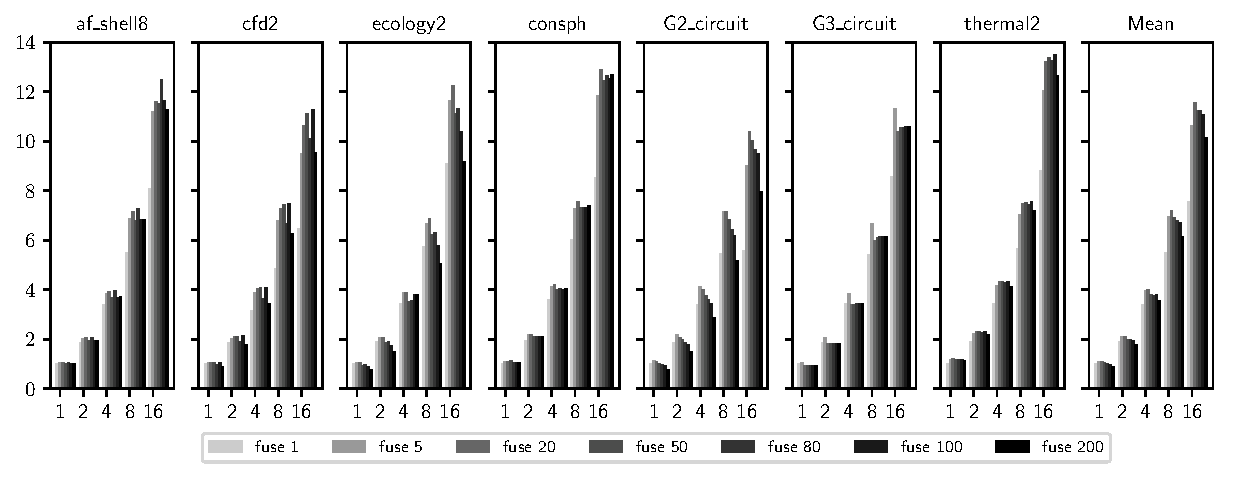
\includegraphics[width=\textwidth, trim={0cm 0 0cm 0},clip]{ifcg/figs/mn3_fuse/cg_speedup_bar_nd.pdf}}
        \caption{Impact of the \emph{FUSE} parameter on IFCG1. The y-axis represents the achieved speedups with respect to the \emph{FUSE}=1 configuration running on 1 core while x-axis represents core counts.}
        \label{fuse}
\end{figure*}

When running on a single core we achieve speedups of 1.12x, 1.12x and 1.09x over the \emph{FUSE} $=1$ configuration when \emph{FUSE} is set to 5, 20 and 50, respectively. 
This modest speedups are due to the reduction of overheads brought by checks for convergence, i. e. computing $Ax_i-b$, which is done once every \emph{FUSE} iterations. 
These small benefits decrease for large \emph{FUSE} values due to the extra iterations the algorithm carries out.  
When the experiments are run on larger core counts the benefits of increasing the \emph{FUSE} value are very significant.
Indeed, we achieve average speedups of 10.44x, 11.15x and 10.99x when \emph{FUSE} is set to 5, 20 and 50 and IFCG1 runs on 16 cores with respect to the sequential run with \emph{FUSE} $=1$.
In general, the benefits of increasing \emph{FUSE} stall at 20 and start to decline when \emph{FUSE} reaches the 200 value.
Matrix-wise, results are very consistent since IFCG1 reaches optimal or very close to optimal performance when \emph{FUSE} $=20$ for 5 matrices: \emph{cfd2}, \emph{ecology2}, \emph{consph}, \emph{G2\_circuit} and \emph{thermal2}. 
Just for the \emph{af\_shell8} and \emph{G3\_circuit} matrices the \emph{FUSE} optimal value is different from 20 (80 in the first case and 5 in the second) although the speedups in these optimal points (12.5x and 11.33x respectively), are very close to the ones achieved by the \emph{FUSE} $=20$ configuration (11.62x and 10.38x).
In general, a \emph{FUSE} value of 20 is the best one for the IFCG1 algorithm.
By conducting the same analysis for IFCG2 we find its optimal \emph{FUSE} parameter to be 20 as well. 

\subsection{Evaluation of the IFCG1 and IFCG2 algorithms against state-of-the-art techniques}
\label{sec:ifcg_alg_comp}
This section provides an evaluation of the parallel speedups achieved by the IFCG1 and the IFCG2 algorithms 
and compares them with 4 state-of-the-art techniques: Preconditioned CG (PCG), Pipelined CG~\cite{ghysels14}, Chronopoulos CG~\cite{chronopoulos89} and Gropp CG~\cite{gropp10}.
Both IFCG1 and IFCG2 run with \emph{FUSE} $=20$, which is the configuration that provides the best performance on average, as shown in section~\ref{sec:ifcg_fuse}.
Figure~\ref{comp} provides a comparison in terms of speedup considering all 6 CG variants.
The x-axis represents the number of cores involved in the parallel run while the y-axis shows the speedups achieved by the different techniques taking the execution time of the Preconditioned CG algorithm on a single core as reference.
The experimental setup is described in Section~\ref{sec:ifcg_setup}.

\begin{figure*}[bhtp]
	\centerline{\includegraphics[width=\textwidth, trim={0.0cm 0 0.0cm 0},clip]{ifcg/figs/mn3_comp/cg_speedup_bar2.pdf}}
	%\centerline{\includegraphics[width=\textwidth, trim={2.5cm 0 2.5cm 0},clip]{figs/mn3_comp/cg_speedup_bar2.pdf}}
	%\centerline{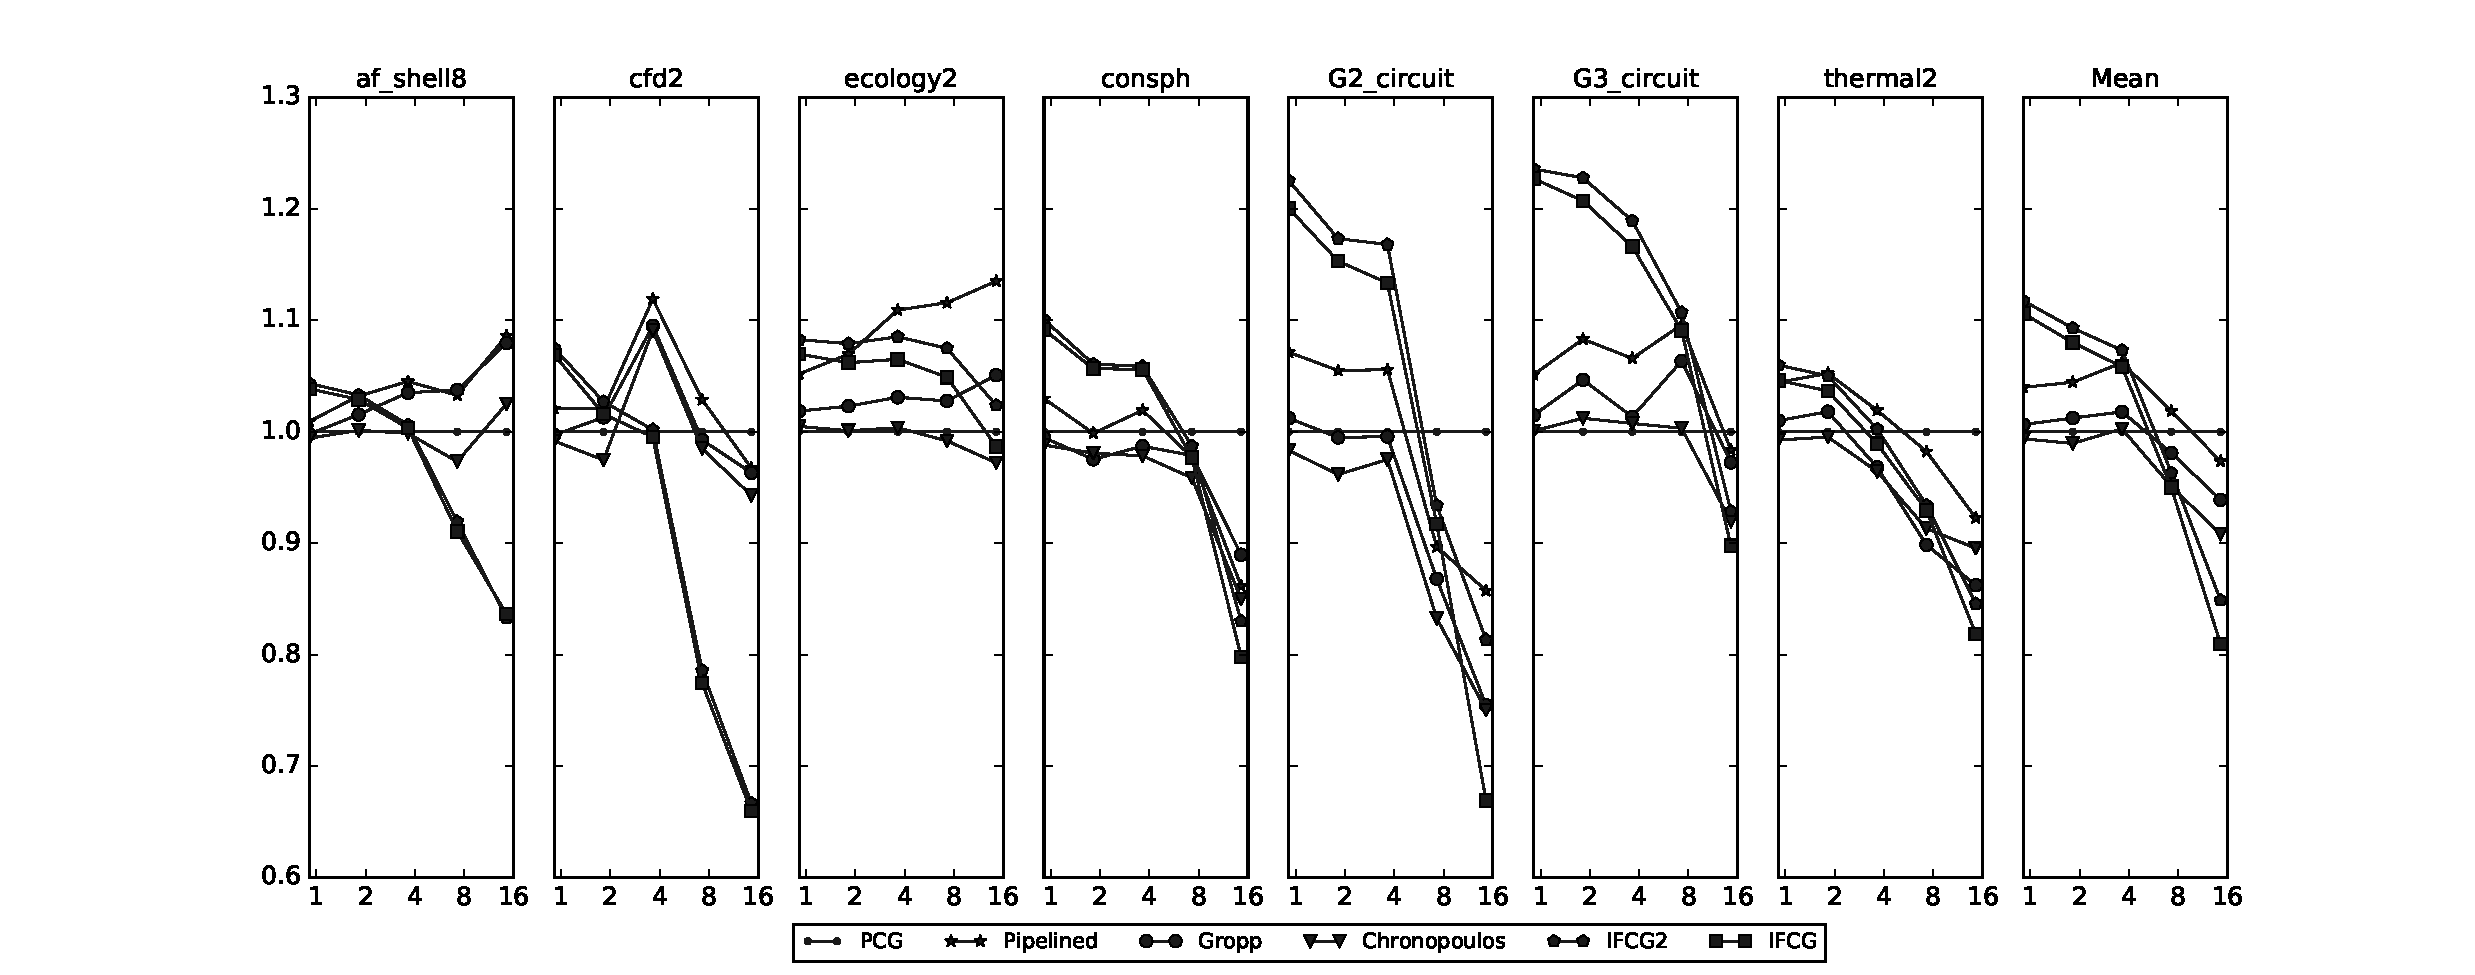
\includegraphics[width=\textwidth, trim={2cm 0 2.5cm 0},clip]{figs/mn3_comp/cg_speedup_lin.pdf}}
	%\vspace{-.75cm}
	\caption{Speedup of all considered CG versions with respect to PCG running on 1 core. The y-axis represents the speedups achieved by the different techniques while x-axis represents core counts.}
	\label{comp}
\end{figure*}

The most dramatic improvements are achieved when applying IFCG1 and IFCG2 to the \emph{af\_shell8} and \emph{cfd2} matrices. 
For these two matrices IFCG1 running on 16 cores achieves speedups of 10.92x and 10.96x while IFCG2 reaches speedups of 9.72x and 9.62x, respectively.
These results are much better than the speedups achieved by the other considered techniques.
Indeed, the speedups achieved by the Preconditioned, Pipelined, Gropp and Chronopoulos variants of the CG algorithm are 9.13x, 8.41x, 8.46x and 8.91x in the case of \emph{af\_shell8} and 6.41x, 6.63x, 6.66x and 6.8x in the case of \emph{cfd2}, respectively.
In the case of the \emph{cfd2} matrix the performance improvements achieved by IFCG1 and IFCG2 are 42.9\% and 41.5\% better than Chronopoulos, the best state-of-art-technique.
IFCG1 provides the highest performance in almost all the cases.
The only exception is \emph{ecology2}. %and \emph{nd24k} matrices. 
In this case, the best speedup on 16 cores is achieved by the Chronopoulos CG (10.98x) although IFCG1 provides a very close speedup of 10.82x when run on 16 cores.
%In the case of the \emph{nd24k} matrix the fastest technique is the Pipelined CG (6.13x), although IFCG1 provides a speedup of 5.35x.
This represents a case where techniques proposed in this paper are not better than the state-of-the-art since the input matrix makes the linear system easily scalable (all CG variants achieve speedups close to 10x with respect to PCG running on a single core when solving the \emph{ecology2} on 16 cores).
% or, \textcolor{red}{oppositely, impossible to scale due its restricted number of rows and columns (\emph{nd24k}).}

%\begin{figure}[bhtp]
%        \centerline{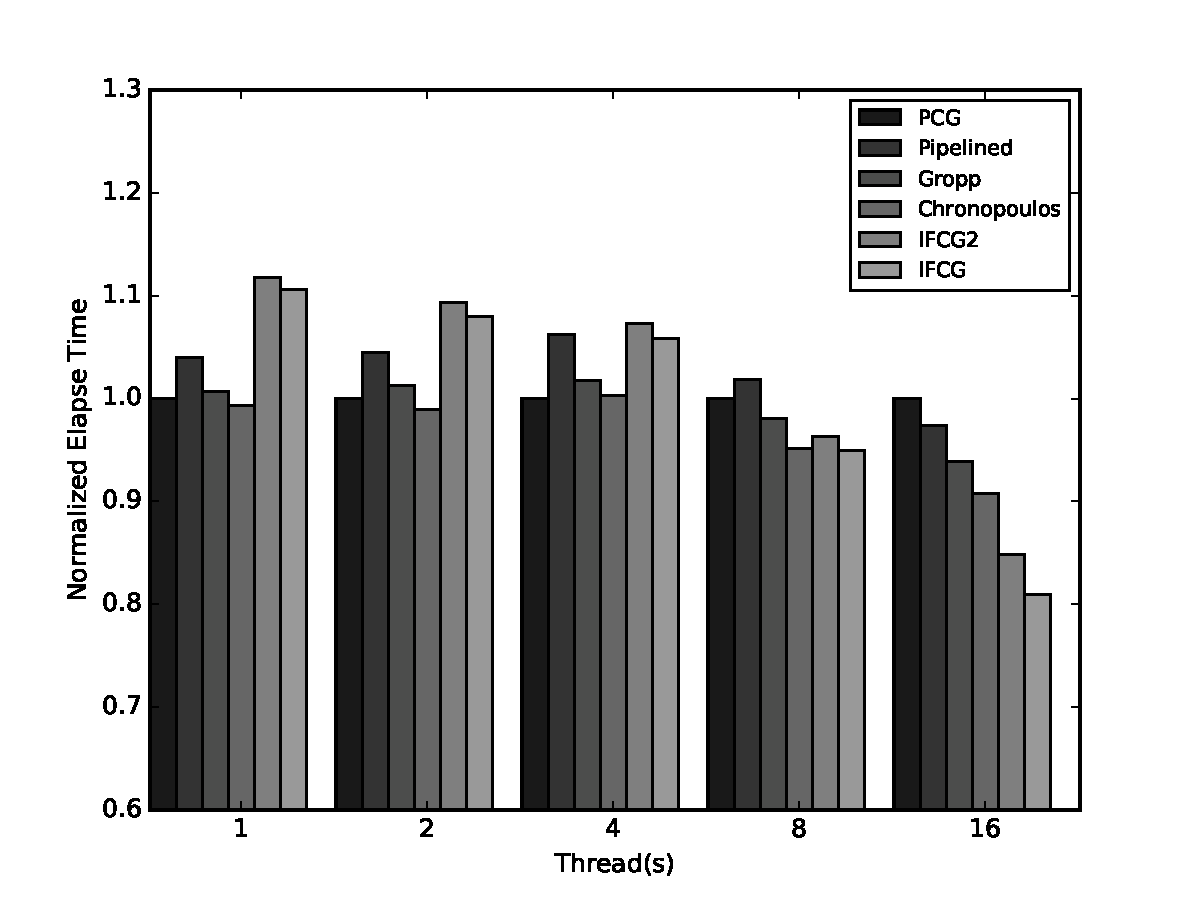
\includegraphics[scale=0.50]{figs/mn3_comp/cg_speedup_bar3.pdf}}
%        \caption{Speedup of all considered CG versions with respect to PCG running on 1 core (top) and the relative performance of all considered CG versions with respect to PCG running on the same amount of cores (bottom). The y-axis represents the speedups achieved by the different techniques while x-axis represents core counts.}
%        \label{comp2}
%\end{figure}

Besides individual observations, the average speedup over the PCG algorithm running in a single core of both IFCG1 and IFCG2 is significantly better than the one achieved by the other CG versions. 
Indeed, we can observe from Figure~\ref{comp} that IFCG1 and IFCG2 reach an average speedup 
when run on 16 cores of 10.06x and 9.64x, respectively.
The other variants achieve speedups of 8.20x (PCG), 8.40x (Pipelined), 8.70x (Gropp) and 8.99x (Chronopoulos) when run on 16 cores.  
On average, IFCG1 and IFCG2 provide 11.8\% and 7.1\% performance improvements over the best state-of-the-art technique (Chronopoulos CG).
Table~\ref{table:iterations} lists the iteration counts for all considered matrices and CG variants.
Due to the residual check done once every \emph{FUSE} iterations the IFCG1 and IFCG2 algorithms are
bound to take more iterations than the other approaches and
indeed they take 16 more iterations on average than the other CG variants. 
This overhead is effectively compensated by overlapping adjacent iterations, as Figure~\ref{comp} demonstrates.

\begin{table}[bhtp]
\centering
\fontsize{9}{9}\selectfont
\resizebox{.80\textwidth}{!}{  
\begin{tabular}{|c|c|c|c|c|c|c|}
\hline 
~ & \textbf{PCG} & \textbf{Chronopoulos} & \textbf{Pipelined} & \textbf{Gropp} & \textbf{IFCG} & \textbf{IFCG2} \\ 
\hline \hline
af\_shell8 & 676 & 676 & 676 & 676 & 680 & 680 \\
\hline
cfd2 & 563 & 563 & 563 & 563 & 580 & 580 \\ 
\hline
ecology2 & 678 & 678 & 678 & 678 & 680 & 680 \\ 
\hline
consph & 912 & 911 & 926 & 911 & 940 & 940 \\ 
\hline
G2\_circuit & 430 & 430 & 430 & 430 & 440 & 440 \\ 
\hline
G3\_circuit & 428 & 428 & 428 & 428 & 480 & 480 \\ 
\hline
%nd24k & 591 & 591 & 590 & 591 & 600 & 600 \\ 
%\hline
thermal2 & 2076 & 2076 & 2077 & 2076 & 2080 & 2080 \\ 
\hline
Average & 794 & 794 & 796 & 794 & 810 & 810 \\ 
\hline
\end{tabular}
}
\vspace{0.2cm}
\caption{Iteration counts of all considered methods and matrices. \emph{FUSE} = 20 for IFCG1 and IFCG2}
\label{table:iterations}
\vspace{-0.5cm}
\end{table}

\subsection{Visualizing The Overlap Pattern}
\label{sec:ifcg_visualization}
The main reason behind the good behavior of IFCG1 and IFCG2 in terms of performance is their capacity to overlap different iterations and 
this section aims to provide a visual proof of this overlap.
Figure~\ref{paraver} displays three 16-core runs composed of 19 iterations.
On top of Figure~\ref{paraver} we represent a Pipelined CG execution while IFCG1 is shown in the middle and IFCG2 at the bottom.
In the y-axis we represent the 16 threads involved in the parallel run while in the x-axis we show time.
The three represented algorithms are applied to the \textit{af\_shell8} matrix.
In all three views the iterations are marked by distinct colors and all are trimmed for the same
time duration (the duration of the pipelined CG since it takes the longest time).
The white gaps in Figure~\ref{paraver} represent either idle time or system software activity.


Boundaries between iterations are clearly marked by white gaps in the Pipelined CG representation of Figure~\ref{paraver}.
Computations belonging to the same iteration are clearly executed in isolation by the Pipelined CG algorithm
while this lock-step execution mode is not present in the IFCG1 and IFCG2 representations.
For these two cases computations belonging to different iterations are overlapped in a way that only their color identifies the iteration they belong to.
There are some small regions represented in white in the IFCG1 and IFCG2 parallel runs that are overlapped with iterations, which account for system software activity. The idle time is almost completely eliminated.
The white areas overlapped with the first iteration of IFCG1 and IFCG2 represent computations belonging to previous iterations while the large white areas that appear after the 19 iterations mean that the parallel execution has already finished.

\begin{figure*}[!bhtp]
        \centerline{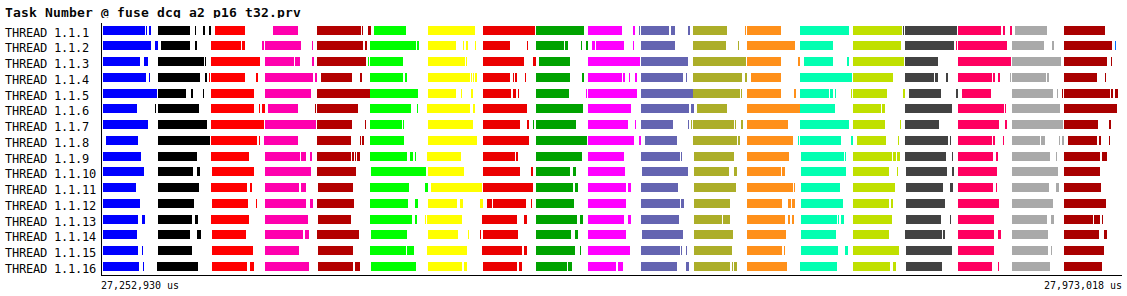
\includegraphics[scale=0.40]{ifcg/figs/traces/alg2.png}}
        \centerline{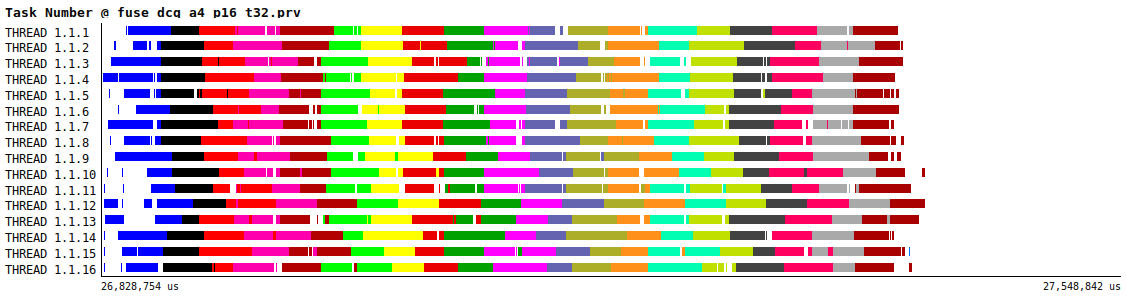
\includegraphics[scale=0.40]{ifcg/figs/traces/alg4.png}}
        \centerline{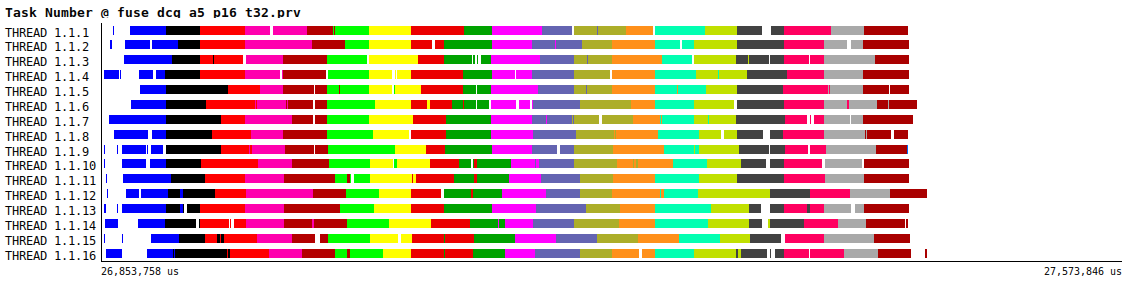
\includegraphics[scale=0.40]{ifcg/figs/traces/alg5.png}}
        \caption{Visualization of 19-iteration runs on 16 cores of Pipelined CG (top), IFCG1 (middle) and IFCG2 (bottom). The input matrix is \textit{af\_shell8}}
        \label{paraver}
\end{figure*}

\subsection{Tolerance to System Noise}
HPC infrastructures frequently get their performance severely degraded by system noise or jitter, which is caused by factors like OS activity, network sharing effects or other phenomena~\cite{Morari11}.
Although the effects of system jitter may be negligible as long as they are kept at the local scale, parallel operations like reductions or synchronizations are known to strongly amplify its effects by propagating jitter across the whole parallel system~\cite{Hoefler10}.
Since algorithms IFCG1 and IFCG2 presented in this paper perform much less reductions or synchronization operations than the Preconditioned CG or the Chronopoulos CG algorithms, they are much more tolerant to jitter effects. 
To evaluate this additional advantage of IFCG algorithms, this section compares the performance of these 4 algorithms (Preconditioned CG, Chronopoulos CG, IFCG1 and IFCG2) on a noisy regime.
The Gropp and Pipelined versions of CG are not considered in this section since, as Figure~\ref{comp} demonstrates, their behavior is between the one displayed by PCG and Chronopoulos.

We run the 4 algorithms mentioned above on 16 cores considering the input matrices and the experimental setup described in Section~\ref{sec:ifcg_setup} and we inject uniformly distributed random noise with an amplitude of 10$\mu$s and frequencies of 8kHz and 2kHz.
Such noise regimes are close to the measured ones on real systems (1kHz and 25$\mu$s~\cite{Ferreira08}) and produce, on average, overheads of 8\% ($8\cdot10^3 \cdot 10^{-5} = 0.08$) and 2\% in sequential computations, respectively.
Therefore, any extra overhead suffered by parallel applications under these noise regimes is brought by amplification effects due to parallel synchronization or reduction operations.
Parallel executions may also filter out noisy events that take place during idle execution phases.

In Figure~\ref{resiliency} we show the elapsed time running on 16 cores of the Preconditioned CG, Chronopoulos CG, IFCG1 and IFCG2 under a noiseless, a 10$\mu$s-2kHz and a 10$\mu$s-8kHz noise regimes. 
The y-axis displays the execution time normalized to the Preconditioned CG execution without noise and the x-axis shows the obtained results per matrix plus their average values. 
On average, the Preconditioned and the Chronopoulos CG algorithms suffer degradation of 19.0\% and 14.6\% of their execution time, respectively under the 10$\mu$s-8kHz noise regime. 
They are much larger than the 8\% degradation expected to be suffered by purely sequential applications, which implies that noise is amplified by parallel operations like reductions or synchronizations.
In contrast, IFCG1 and IFCG2 suffer much milder degradation of just 6.2\% and 6.9\%, respectively, when exposed to 10$\mu$s-8kHz noise.
IFCG1 has a 1.18x speedup over Chronopoulos under the 10$\mu$s-8kHz, that is, it runs 18.0\% faster.
Interestingly, both IFCG algorithms run faster under this noisy regime than their state-of-the-art counterparts under the noiseless regimes.
In Figure~\ref{resiliency} we also show results considering the 10$\mu$s-2kHz scenario.
For this case, the Preconditioned and the Chronopoulos CG algorithms suffer degradation of 6.1\% and 5.1\% of their execution time, respectively.
In contrast, IFCG1 and IFCG2 suffer milder degradation of just 1.1\% and 1.7\%, respectively.

\begin{figure*}[!bhtp]
        \centerline{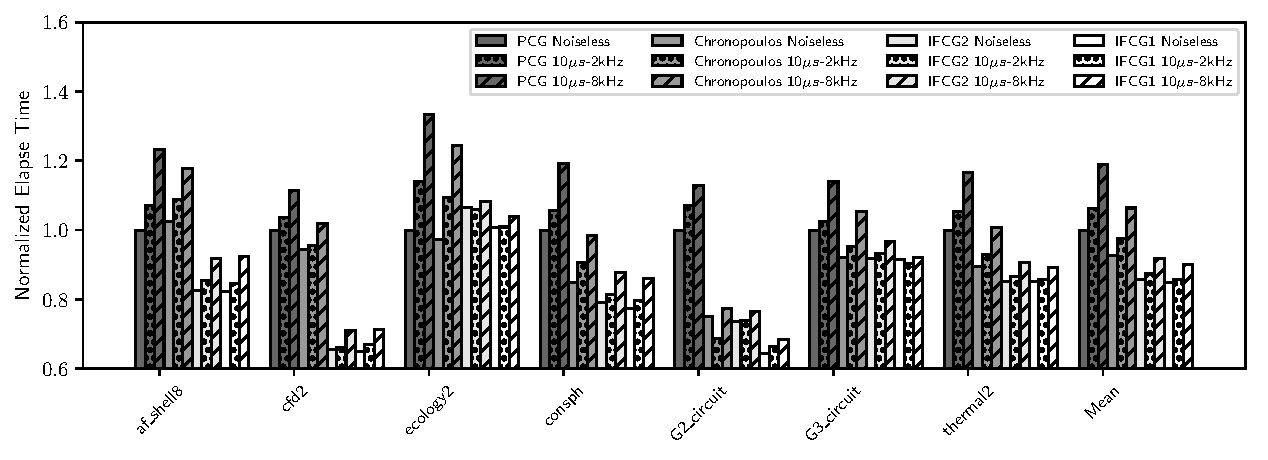
\includegraphics[width=\textwidth]{ifcg/figs/resiliency/resilient_unified.pdf}}
        \caption{Behavior of different variants of CG running on 16 cores under noiseless, 10$\mu$s-2kHz and 10$\mu$s-8kHz noise regimes.}
        \label{resiliency}
\end{figure*}


